\chapter{State of the Art}\label{ch:state-of-the-art}

\section{Problem 1 - Tactile Perception}\label{sec:lit-rev-problem-1}

Based on the contact model categories described above, the most representative is \gls{sf} since these can provide descriptions of the contact surface topology, and thus enable the solving of the \gls{iep} by deriving surface features for pose estimation. Furthermore these represent friction forces and moments which in needed in order to manipulate objects in-hand and ensuring force closure.\medskip

% \begin{center}
%     \renewcommand{\arraystretch}{1.2}
%     \begin{minipage}{.48\linewidth}
%         \vspace{0pt}
%         \centering
%         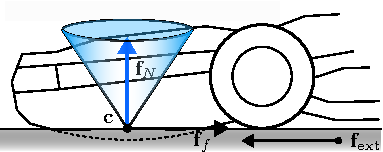
\includegraphics[width=.95\textwidth]{chapters/modeling/fig/friction-cone-schematic.pdf}
%     \end{minipage}%
%     \hfill%
%     \begin{minipage}{.48\linewidth}
%         \vspace{0pt}
%         \centering
%         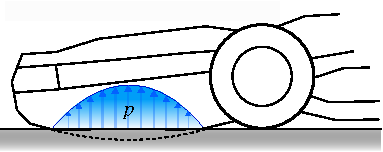
\includegraphics[width=.95\textwidth]{chapters/modeling/fig/contact-surface.pdf}
%     \end{minipage}%
%     %    
%     \vspace{15pt}
%     %
%     \begin{minipage}[t]{.48\linewidth}
%         \vspace{0pt}
%         \captionsetup{type=figure}
%         \captionof{figure}{Single point contact model between compliant manipulator surface and object surface.}
%         \label{fig:contact-single-point}
%     \end{minipage}%
%     \hfill%
%     \begin{minipage}[t]{.48\linewidth}
%         \vspace{0pt}
%         \captionsetup{type=figure}
%         \captionof{figure}{Contact model of the pressure distribution $p(r)$ caused by the increased force applied from the \gls{ee}'s finger to the object.}
%         \label{fig:contact-surface}
%     \end{minipage}%
% \end{center}


% subcategories of sf models
Within the category of \gls{sf} models a method fit for this project's use case is to be chosen to solve problem \ref{prob:1}. \gls{sf} models can furthermore be divided up into three different categories: \gls{aebm}, \gls{efm} and \gls{fem}~\cite{a-modified-elastic-foundation-contact-model-for-application-in-3d-models-of-the-prosthetic-knee}. \medskip

% reformulate
\gls{aebm} are theoretical formulations of elastic contact areas and the stresses on both the surfaces and the sub-surfaces of the contacting bodies. These types of formulations however are often restricted to describing simple contact geometries. The first of such models was introduced by Heinrich Rudolf Hertz in 1882~\cite{on-the-contact-of-rigid-elastic-solids-and-on-hardness} and is still used for simple contact cases. In the formulation of the Hertzian contact model two assumptions are made: Objects in contact are made of linear elastic materials and only small contact deformations occur compared to the dimension of object. However, robotic \gls{ee} fingertips are often made of nonlinear elastic materials and for that reason the Hertzian contact model does not represent the type of contact in this project~\cite[Chapter 37]{handbook-of-robotics}. To improve on the Hertzian model, a more generic formulation can be made which extends the model from linear to nonlinear elastic contacts~\cite{modeling-of-contact-mechanics-and-friction-limit-surfaces-for-soft-fingers-in-robotics-with-experimental-results}~\cite{the-haptic-and-perceptional-characteristics-of-an-anthropomorphic-curved-soft-finger-structure}. This power-law formulation subsumes the Hertzian contact theory while assuming a circular contact area. Other models have been purposed which combine the descriptions of both friction-contact and the shear-torsion as experienced by the bodies~\cite{the-sliding-of-robot-fingers-under-combined-torsion-and-shear-loading}. \medskip

However, in order to more accurately describe the contacts involving robot fingers, viscoelastic soft contact model appear more relevant due to such fingers often being made of materials which show viscoelastic properties e.g., rubber, silicone and polymers. Simple models such as  Kelvin-Voigt's~\cite{viscoelasticity} and Maxwell's~\cite{on-the-dynamical-theory-of-gases} models describe the interaction between strain and stress as a spring damper system in a serial or in a parallel configuration respectively. Models which expand on this idea describe the reacting force as the product of the temporal and the elastic response, while incorporating previous stress responses~\cite{mechanical-properties-and-active-remodeling-of-blood-vessels}. To simplify this formulation alternatives have been developed to assume no past stress~\cite{modeling-of-viscoelastic-contacts-and-evolution-of-limit-surface-for-robotic-contact-interface}~\cite{characteristics-of-contact-and-limit-surface-for-viscoelastic-fingers}~\cite{effect-of-layer-compliance-on-frictional-behavior-of-soft-robotic-fingers}. Upon these, more modern techniques have been developed which has seen use in similar use cases as the ones of interest in this project. 
% AEBM modern method 2 - A new algorithm for computing the indentation of a rigid body - reformulate - are frictionless MIM (matrix inversion).
One method attempts to expand the description of contacts between rigid indentors and elastic half-spaces, using the \gls{mim} as introduced by Kalker~\cite{on-the-contact-problem-in-elastostatics}, to viscoelastic half-spaces as well. Assuming the surfaces are frictionless, the relationship is described in terms of the pressure distribution, the resultant force on the indenter and the penetration~\cite{a-new-algorithm-for-computing-the-indentation-of-a-rigid-body-of-arbitrary-shape-on-a-viscoelastic-half-space}.
% AEBM modern method 3 - BC's Formulation
Attempts involving solutions to Boussinesq's problem for polynomial pressures acting over polygonal domains~\cite{a-general-approach-to-the-solution-of-boussinesqs-problem-for-polynomial-pressures-acting-over-polygonal-domains} have also been developed and modernized by combining it with Cerruti's solution~\cite{a-boussinesq-cerruti-solution-set-for-constant-and-linear-distribution-of-normal-and-tangential-load-over-a-triangular-area}. However due to numerical singularities being present, modifications are made to threshold the model. For a more complete description without singularities, Love's formulation has been added leading to a more accurate analytical representation but with the cost of an increased computational complexity~\cite{contact-modelling-and-tactile-data-processing-for-robot-skins}. In order for these Boussinesq based approaches to be representative two assumptions are made 1) There exists a linear relation between stress and strain, referred to as deformation, and 2) strains are infinitesimal~\cite[Chapter 6]{the-linearized-theory-of-elasticity}. \medskip

\gls{efm} are methods developed to build upon \gls{aebm} by allow a simple discrete contact calculation in more general surface geometries. Here the deformable part of the contact as a layer over a rigid base is modelled along with a series of discrete and independent springs in the contact normal. A widely used example of this method is the Winkler's elastic foundation model~\cite{kl-johnson-and-contact-mechanics}, which have been used structural engineering for modeling different properties of beams such as stability~\cite{stability-of-a-timoshenko-beam-resting-on-a-winkler-elastic-foundation}, vibrations and buckling~\cite{vibrations-and-buckling-of-a-beam-on-a-variable-winkler-elastic-foundation}. Other \gls{efm} methods have shown accurate modeling performance when applied within the field of medical engineering. Here a comparative study between \gls{aebm}, \gls{efm} and \gls{fem} demonstrate the suggested modified \gls{efm} performs better than the alternatives in 3D knee models when predicting prosthetic knee performance~\cite{a-modified-elastic-foundation-contact-model-for-application-in-3d-models-of-the-prosthetic-knee}. A different method attempts to attain vivo contact pressure predictions for improved knee replacement designs~\cite{experimental-evaluation-of-an-elastic-foundation-model-to-predict-contact-pressures-in-knee-replacements}
Within the field of robotics \gls{efm} have provided solutions to problems such as slip~\cite{the-sliding-of-robot-fingers-under-combined-torsion-and-shear-loading}, compliance, sliding~\cite{quasistatic-manipulation-with-compliance-and-sliding}~\cite{practical-force-motion-models-for-sliding-manipulation}, stiffness and contact mechanics~\cite{stiffness-and-contact-mechanics-for-soft-fingers-in-grasping-and-manipulation} of humanoid grippers.
One such method derives friction constraints based on general expressions for non-planar contacts of elastic bodies, where the local geometry and structure of the objects in contact are taken into account. Using these, a linear complementary problem is formulated and solved, resulting in the normal and frictional forces applied at each contact, as well as the relative velocity of the bodies involved~\cite{soft-finger-model-with-adaptive-contact-geometry-for-grasping-and-manipulation-tasks}. \medskip

\gls{fem} are popular general tools for solving PDE~\cite{history-of-finite-element-method:-a-review} and have seen contact applications in a wide range of engineering discipline due to the assumptions made in \gls{aebm} and \gls{efm} not being applicable in these cases. A great number of these cases exist within the manufacturing industry~\cite{examples-of-fem-application-in-manufacturing-technology} whereas one example is the metal forming processes. Specifically the the estimation of wheel rail profiles~\cite{contact-mechanics-analysis-of-measured-wheel-rail-profiles-using-the-finite-element-method} has been addressed using \gls{fem} due to the estimation of contacts over a greater surface is needed than what is assumed in \gls{aebm} and \gls{efm}. Other applications such as quality control through sliding wear estimation~\cite{simulating-sliding-wear-with-finite-element-method}, analysis of the responses of fully coupled thermo-elasto-plastic solids in contact~\cite{a-finite-element-procedure-for-the-analysis-of-thermo-mechanical-solids-in-contact} and performing diagnostics of failures in induction motors~\cite{induction-motors-fault-diagnosis-using-finite-element-method:-a-review}. Due to the complexity of modeling the contacts within robotics, \gls{fem} have become a popular choice and enabled tactile applications such as \gls{cobot} tactile skin for ensuring collaborative behavior when in contact~\cite{soft-robot-skin-with-conformal-adaptability-for-on-body-tactile-perception-of-collaborative-robots}, performance estimation of new tactile sensor technologies~\cite{design-and-experimental-research-of-robot-finger-sliding-tactile-sensor-based-on-fbg} and evaluating complex contact types by extending simulations and analysis systems~\cite{grasp-analysis-using-deformable-fingers}.
The modelling complexity has furthermore inspired using \gls{fem} as ground truth results when synthesizing machinelearning data in simulations for deep learning models, which has enabled execution speeds 75 times greater than simply evaluating \gls{fem}~\cite{sim-to-real-for-robotic-tactile-sensing-via-physics-based-simulation-and-learned-latent-projections} 
~\cite{interpreting-and-predicting-tactile-signals-via-a-physics-based-and-data-driven-framework}
~\cite{ground-truth-force-distribution-for-learning-based-tactile-sensing:-a-finite-element-approach}. \medskip

The contact model chosen for this project is the \gls{aebm} Love's formulation due to its capabilities of representing contact surface displacements with great precision~\cite{contact-modelling-and-tactile-data-processing-for-robot-skins}.

\section{Problem 2 - Pose Estimation}\label{sec:lit-rev-problem-2}

\section{Problem 3 - In-Hand Manipulation}\label{sec:lit-rev-problem-3}